\section{ST-structures}
\label{sec:ST-structures}
    
    ST-structures are first introduced by Johansen in \cite{Johansen16STstruct}. They are an extension of \emph{configuration structures} \cite{GlabbeekP95config} and \emph{unrestricted} event structures \cite{GlabbeekP09configStruct}. 
    
    \begin{figure}[ht]
        \centering
        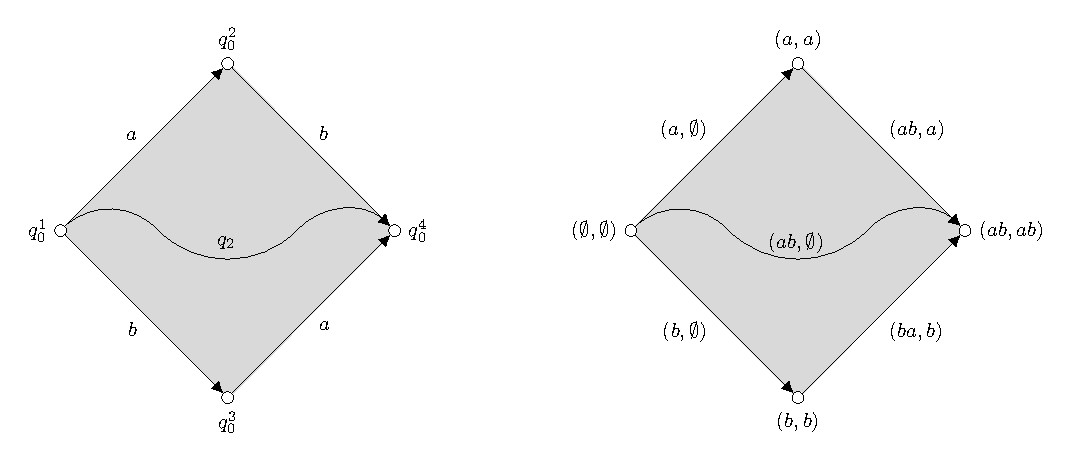
\includegraphics[scale=0.9]{master_thesis/Figures/3.An-introduction-to-non-interleaving-models-for-concurrency/ST-structure/st-structure-interleaving-square.pdf}
         \captionof{figure}[ST-structure]{Example of a higher-dimensional automaton with two concurrent events labelled by $a$ and $b$: with a geometrical picture of the higher-dimensional automaton (left) and of the ST-structure (right).}
        \label{fig:st-structure-interleaving-square}
    \end{figure}
    
    In the case of configuration structures and event structures, we have that the classical notion of concurrency, causality, and conflict are not interdefinable. In the case of higher-dimensional automata these notions can be interdefinable. In Chapter \ref{chap:Relationship with other models of true concurrency}, we relate ST-structures to higher-dimensional automata by identifying a corresponding class of ST-structures with the particular property of \emph{adjacent-closure}. With the adjacent-closure property, ST-structures are able to capture the higher-dimensional case of the notions of concurrency, causality and conflict. We will use the same notation and definitions as Johansen in \cite{Johansen16STstruct}.
    
    \begin{definition}[ST-configuration \cite{Johansen16STstruct}]
        \label{def:st-configuration}
        An ST-configuration over some set $E$ of events is a pair of finite sets ($\mathcal{S},\mathcal{T}$) ($\mathcal{S}, \mathcal{T} \subseteq E$) respecting the property:
        
        \begin{center}
            (start before terminate) $\mathcal{T} \subseteq \mathcal{S}$.
        \end{center}
    \end{definition}
    
    In the following, $\mathcal{S}$ contains the events that have started and $\mathcal{T}$ the events that have terminated. In the current ST-configuration, we see the events $\mathcal{S} \setminus \mathcal{T}$ as being executed \emph{concurrently}. We will call $| \mathcal{S} \setminus \mathcal{T} |$ the concurrent degree of this ST-configuration, similar to how we defined dimensions for higher-dimensional automata. The notion of degree, and dimension, is the main characteristic captured by ST-structures which is found in higher-dimensional automata, but not found in classical event-based models like configuration structures or event structures. In ST-structures, an event can be seen to have started and not terminated yet, capturing the notion of \emph{duration}.
    
    \begin{definition}[ST-structures \cite{Johansen16STstruct}]
        \label{def:st-structures}
        An ST-configuration structure (also called ST-structure) is a tuple $ST$ = ($E, ST, l$) with ST a set of ST-configurations over $E$ satisfying the constraint:
        
        \begin{center}
            if ($\mathcal{S},\mathcal{T}$) $\in$ ST then ($\mathcal{S},\mathcal{S}$) $\in$ $ST$,
        \end{center}
    
    and $l:E$ $\rightarrow \Sigma$ a labelling function with $\Sigma$ the set of labels. we often omit the set of events $E$ from the notation when there is no danger of confusion.
    \end{definition}
    
    Intuitively, the constraint above ensures that every event that is represented, and that has also started, has to be terminated. We denote $\mathbb{S} \mathbb{T}$ as the set of all ST-structures.
    
    \begin{definition}[Stable ST-structures \cite{Johansen16STstruct}]
        \label{def:stable st-structures}
        A ST-structure ($E, ST,l$) is called:
        
        \begin{enumerate}
            \item rooted iff ($\emptyset$,$\emptyset$) $\in ST$;
            \item connected iff for any non-empty ($\mathcal{S},\mathcal{T}$) $\in ST$, either \\
            $\exists$e $\in$ $\mathcal{S}$ : ($\mathcal{S}\setminus e, \mathcal{T}$) $\in ST$ or $\exists$e $\in \mathcal{T}$ : ($\mathcal{S}, \mathcal{T}\setminus e$) $\in ST$;
            \item closed under bounded unions iff for any ($\mathcal{S},\mathcal{T}$),($\mathcal{S}',\mathcal{T}'$),($\mathcal{S}'',\mathcal{T}''$) $\in ST$ if ($\mathcal{S},\mathcal{T}$) $\cup$ ($\mathcal{S}',\mathcal{T}'$) $\subseteq$ ($\mathcal{S}'',\mathcal{T}''$) then ($\mathcal{S},\mathcal{T}$) $\cup$ ($\mathcal{S}',\mathcal{T}'$) $\in ST$;
            \item closed under bounded intersection iff for ($\mathcal{S},\mathcal{T}$),($\mathcal{S}',\mathcal{T}'$),($\mathcal{S}'',\mathcal{T}''$) $\in ST$ if ($\mathcal{S},\mathcal{T}$) $\cup$ ($\mathcal{S}',\mathcal{T}'$) $\subseteq$ ($\mathcal{S}'',\mathcal{T}''$) then ($\mathcal{S},\mathcal{T}$) $\cap$ ($\mathcal{S}',\mathcal{T}'$) $\in ST$;
        \end{enumerate}
        
        a ST-structure is called stable iff it is rooted, connected, and closed under bounded unions and intersections.
    \end{definition}
    
    Stable ST-structures satisfy the properties of being rooted, connected, and closed under bounded unions and intersections. Rooted is where the ST-structure has a ST-configuration that has no events running or terminated. Connected means that for every non-empty configuration, that is, an event has terminated or is running, there must exist another configuration where that event has not started, or terminated, yet. Both closed under bounded union and intersection, are operations that provide configurations that already exist in the ST-structure.
    

    \begin{definition}[Stable ST-structures \cite{Johansen16STstruct}]
    \label{def:st-steps}
        A step between two ST-configurations is defined as either:
        
        \begin{description}
            \item[s-step] $(\mathcal{S},\mathcal{T})\transitions{e}(\mathcal{S}',\mathcal{T}')$ when $\mathcal{T}=\mathcal{T}'$, $\mathcal{S} \subset \mathcal{S}'$, $\mathcal{S}' \setminus \mathcal{S}=\{e\}$; or
            \item[t-step] $(\mathcal{S},\mathcal{T})\transitiont{e}(\mathcal{S}',\mathcal{T}')$ when $\mathcal{S}=\mathcal{S}'$, $\mathcal{T} \subset \mathcal{T}'$, $\mathcal{T}' \setminus \mathcal{T}=\{e\}$.
        \end{description}
        When the type is unimportant we denote a step by \, $\transition{e}$ \, for \, $\transitions{e}\cup\transitiont{e}$. A \emph{path} of a ST-structure, denoted $\pi$, is a sequence of steps, where the end of one is the beginning of the next, in other words,
        
        \[
            \pi\defequal(\mathcal{S},\mathcal{T})\transition{e}(\mathcal{S}',\mathcal{T}')\transition{e'}(\mathcal{S}'',\mathcal{T}'')\dots
        \]

        A path is \emph{rooted} if it starts in $(\emptyset,\emptyset)$.
    \end{definition}
    
    A \emph{computational interpretation} for ST-structures is defined by defining simple steps between ST-configurations, similar to interpretations for other concurrency models like configurations structures. However in \cite[Theorem 3.10]{Johansen16STstruct}, the computational interpretation for ST-structures is shown to be more fine-grained than other models such as configuration structures and event structures, since ST-structures can capture the notion of \emph{duration}.
    
    The notion of duration is similar to what is captured in higher-dimensional automata, but from a state-based perspective. Hence, ST-structures are capable of showing a natural sequence of \emph{observable information} as ST-traces in a similar manner as higher-dimensional automata \cite[Section 7.3]{Glabbeek06HDA}. Following the notion of Johansen in \cite{Johansen16STstruct}, we may consider ST-structures the richest formalisation of observable content for concurrent systems.
    
    \begin{definition}[Paths and traces \cite{Johansen16STstruct}]
        \label{def:paths and traces}
        A path of a ST-structure, denoted $\pi$, is a sequence of steps, where the end of one is the beginning of the next, that is,
        
        \begin{center}
            $\pi \triangleq$ $(\mathcal{S}_{0},\mathcal{T}_{0})\xrightarrow{a}(\mathcal{S}_{1},\mathcal{T}_{1})\xrightarrow{b}(\mathcal{S}_{2},\mathcal{T}_{2})$...    
        \end{center}
        
        A path is rooted if it starts in ($\emptyset$,$\emptyset$). The ST-trace of a rooted path $\pi$, denoted $st(\pi)$, is the sequence of labels of the steps of $\pi$ where each label is annotated as $a^{0}$ if it labels an s-step or as $a^{n}$ if it labels a t-step. where $n \in  \mathbb{N}$ is determined by counting from the beginning the number of steps until the s-step that has added the event \emph{e} to the $\mathcal{S}$ set, which \emph{e} being the event that has been added to $\mathcal{T}$ in the current t-step.
    \end{definition}
    
    If we consider rooted and connected ST-structures, then the notion of ST-trace matches with the one in \cite[Definition 2.5]{GlabbeekV97splitting} and in \cite[Section 7.3]{Glabbeek06HDA}. Below we define the notion of concurrency and causality for a particular ST-configuration as Johansen in \cite{Johansen16STstruct}.
    
    \begin{definition}[Concurrency and causality \cite{Johansen16STstruct}]
        \label{def:ST concurrency and causality}
        For a particular ST-configuration ($\mathcal{S},\mathcal{T}$) $\in \cat{ST}$ where $e, e' \in \mathcal{S}$ satisfies
        
        \begin{itemize}
            \item \textbf{Concurrency:} $e \parallel e'$ iff there exists $(\mathcal{S}',\mathcal{T}') \subseteq (\mathcal{S},\mathcal{T})$ such that
            \begin{itemize}
                \item $(\mathcal{S}',\mathcal{T}') \in \cat{ST}$, and
                \item $\{e,e'\} \subseteq \mathcal{S}' \setminus \mathcal{T}'$.
            \end{itemize}
            \item \textbf{Causality:} $e < e'$ iff $e \neq e'$ and for any $(\mathcal{S}',\mathcal{T}') \subseteq (\mathcal{S},\mathcal{T})$ such that
            \begin{itemize}
                \item $(\mathcal{S}',\mathcal{T}') \in \cat{ST}$, and
                \item $e' \in \mathcal{S}' \Rightarrow e \in \mathcal{T}'$.
            \end{itemize}
        \end{itemize}
    \end{definition}
    
    \emph{Concurrency} for ST-structures is satisfied if we can find a ST-configuration where two events have started, not yet terminated, and is persistent throughout an execution. Other event-based models such as event structures represent concurrency as having events that are not in conflict and not partial ordered. ST-configurations represent concurrency by providing information about the currently concurrent events. 
    
    \emph{Causality} for an ST-configurations is similar to the way causality is defined as a partial order for configuration structures, such that  causality is a local definition for an ST-configuration.
    
    For an arbitrary ST-structure, concurrency and causality are not interdefinable such that concurrency is the complement of causality, as in the standard way \cite[Definition 5.6]{GlabbeekG01refinement}. If we consider well behaved ST-structures such as stable ST-structures, then concurrency and causality can be seen as interdefinable in the standard way.
    
    \begin{definition}[Conflict \cite{Johansen16STstruct}]
        \label{def:ST-structure conflict}
        For a ST-structure ST the notion of global conflict is defined as a predicate over sets of events $E' \subseteq E$:
        
        \begin{center}
            $\# E'$ iff $\nexists (\mathcal{S},\mathcal{T}) \in ST$ with $E' \subseteq \mathcal{S}$.
        \end{center}
    \end{definition}
    
    In the following, the ST-structure describes conflicting events as a predicate where conflicting events in a ST-structure can never appear in the same configuration. Conflicting events is defined as a general notion on the whole ST-structure, and is considered to be similar to the standard notion of binary conflict for event structures \cite{winskel95modelsCategory}.

    \begin{definition}[Adjacent-closure \cite{Johansen16STstruct}]
        \label{def:ST adjacent-closure}
        We call a ST-structure ST adjacent-closed if the following are respected:
       
       \begin{enumerate}
           \item if $(\mathcal{S},\mathcal{T}), (\mathcal{S} \cup e, \mathcal{T}), (\mathcal{S} \cup \{e,e'\}, \mathcal{T}) \in ST$, with $(e \neq e') \notin \mathcal{S}$,\\
           then $(\mathcal{S} \cup e', \mathcal{T}) \in ST;$
           \item if $(\mathcal{S},\mathcal{T}), (\mathcal{S} \cup e, \mathcal{T}), (\mathcal{S} \cup e, \mathcal{T} \cup e') \in ST$, with $e \notin S \wedge e' \notin \mathcal{T} \wedge e \neq e'$, \\
           then $(\mathcal{S}, \mathcal{T} \cup e') \in ST;$
           \item if $(\mathcal{S},\mathcal{T}), (\mathcal{S} \cup e, \mathcal{T}), (\mathcal{S}, \mathcal{T} \cup e') \in ST$, with $e' \notin \mathcal{S} \wedge e' \notin \mathcal{T} \wedge e \neq e'$, \\
           then $(\mathcal{S} \cup e, \mathcal{T} \cup e') \in ST;$
           \item if $(\mathcal{S},\mathcal{T}), (\mathcal{S}, T \cup e), (\mathcal{S}, T \cup \{e,e'\}) \in ST$, with $(e \neq e') \notin \mathcal{T}$, \\
           then $(\mathcal{S}, \mathcal{T} \cup e') \in ST;$
       \end{enumerate}
    \end{definition}
    
    In the following, adjacent-closure for ST-structure is related to the definition of higher-dimensional automata, in other words, the precubical identities of higher-dimensional automata. In the definition of \emph{adjacent} \cite[Definition 19]{Glabbeek99invitedCONCUR}, the correlation becomes more visible when looking at the homotopy over higher-dimensional automata. The homotopy over higher-dimensional automata essentially define histories of higher-dimensional automata, see Definition \ref{def:histories-for-HDA}. Similarly, the above adjacent-closure on ST-structures makes sure that the histories of ST-configurations are represented.
    
    \begin{definition}[Morphisms of ST-structures \cite{Johansen16STstruct}]
        \label{def:morphisms of ST-structures}
        A morphism $f: ST \rightarrow ST'$ between two ST-structures ST = ($E, ST, l$) and ST' = ($E', ST', l'$) is defined as a partial function on the events, $f: E \rightarrow E'$ which:
        
        \begin{itemize}
            \item preserves ST-configurations, if ($\mathcal{S},\mathcal{T}$) $\in ST$ then $f(\mathcal{S},\mathcal{T}) = (f(\mathcal{S}),f(\mathcal{T})) \in ST'$,
            \item preserves the labelling when defined, that is, $l'(f(e)) = l(e)$ if $f$ is defined for $e$, and
            \item is locally injective and total, that is, for any ($\mathcal{S}, \mathcal{T}$) $\in ST$ the restriction $f\rest S$ i s injective and total.
        \end{itemize}
    \end{definition}
    
    Morphisms of ST-structures are structure-preserving maps such that if $\mathcal{T} \subseteq \mathcal{S}$ then $f(\mathcal{T}) \subseteq f(\mathcal{S})$. If morphisms are not local and total, then morphisms are not guaranteed to preserve steps as shown by Johansen in \cite[Proposition 2.21]{Johansen16STstruct}.
    
    \begin{definition}[Isomorphic ST-structures \cite{Johansen16STstruct}]
        \label{def:isomorphic-ST-structures}
        A function $f$ is an isomorphism of two ST-configurations ($\mathcal{S},\mathcal{T}$)$f$($\mathcal{S}',\mathcal{T}'$) iff $f$ is a bijection between $\mathcal{S}$ and $\mathcal{S}'$ that agrees on the sets $\mathcal{T}$ and $\mathcal{T}'$ (that is, $f \rest T = \mathcal{T}'$). Two ST-structures ST and ST are isomorphic, denoted $ST \cong ST'$, iff there exists a bijection $f$ on their events that is also a morphism between the two ST-structures. 
    \end{definition}
    
%    By considering morphisms of ST-structures to be bijections, we are able to consider two ST-structures isomorphic.
    
    \begin{definition}[Category of ST \cite{Johansen16STstruct}]
        \label{def:category of ST}
        We can define a category $\allST$ to have objects ST-structures and the morphisms from Definition \ref{def:morphisms of ST-structures} because composition of morphisms is well defined for any ST-structure there exists a unique identity morphism which is the total function taking an event to itself.
    \end{definition}